\documentclass[tikz,border=5mm,12pt]{article}
\usepackage{tikz}
\usepackage{pgfplots}
\usepackage{geometry}
\usetikzlibrary{shapes.geometric, arrows, calc, angles, positioning}


% define tikz nodes
\tikzstyle{table} = [rectangle, text centered, minimum width=3cm,
	minimum height=4.5cm, draw=black, fill=black!10]
\tikzstyle{kitchen} = [rectangle, text centered, draw=black, 
minimum width=2cm, minimum height=8cm, fill=black!10]


% define tikz arrows
\tikzstyle{arrow} = [<->, >=stealth, thick]
\tikzstyle{arrow-r} = [<->, >=stealth, thick]

% define environment for legend
\newenvironment{legend}[1][]{
	\begingroup
	\csname pgfplots@init@cleared@structures\endcsname
	\pgfplotsset{#1}}
{\csname pgfplots@createlegend\endcsname
	\endgroup
}

% definition to insert numbers
\pgfkeys{/pgfplots/letter in legend/.style={%
		/pgfplots/legend image code/.code={%
			\node [draw=black, circle, fill=blue!10, inner sep=0.5pt] at (0.295,-0.0225){#1};
		},%
	},
}

% make legend available
\def\addlegendimage{\csname pgfplots@addlegendimage\endcsname}

\begin{document}
\pagestyle{empty}

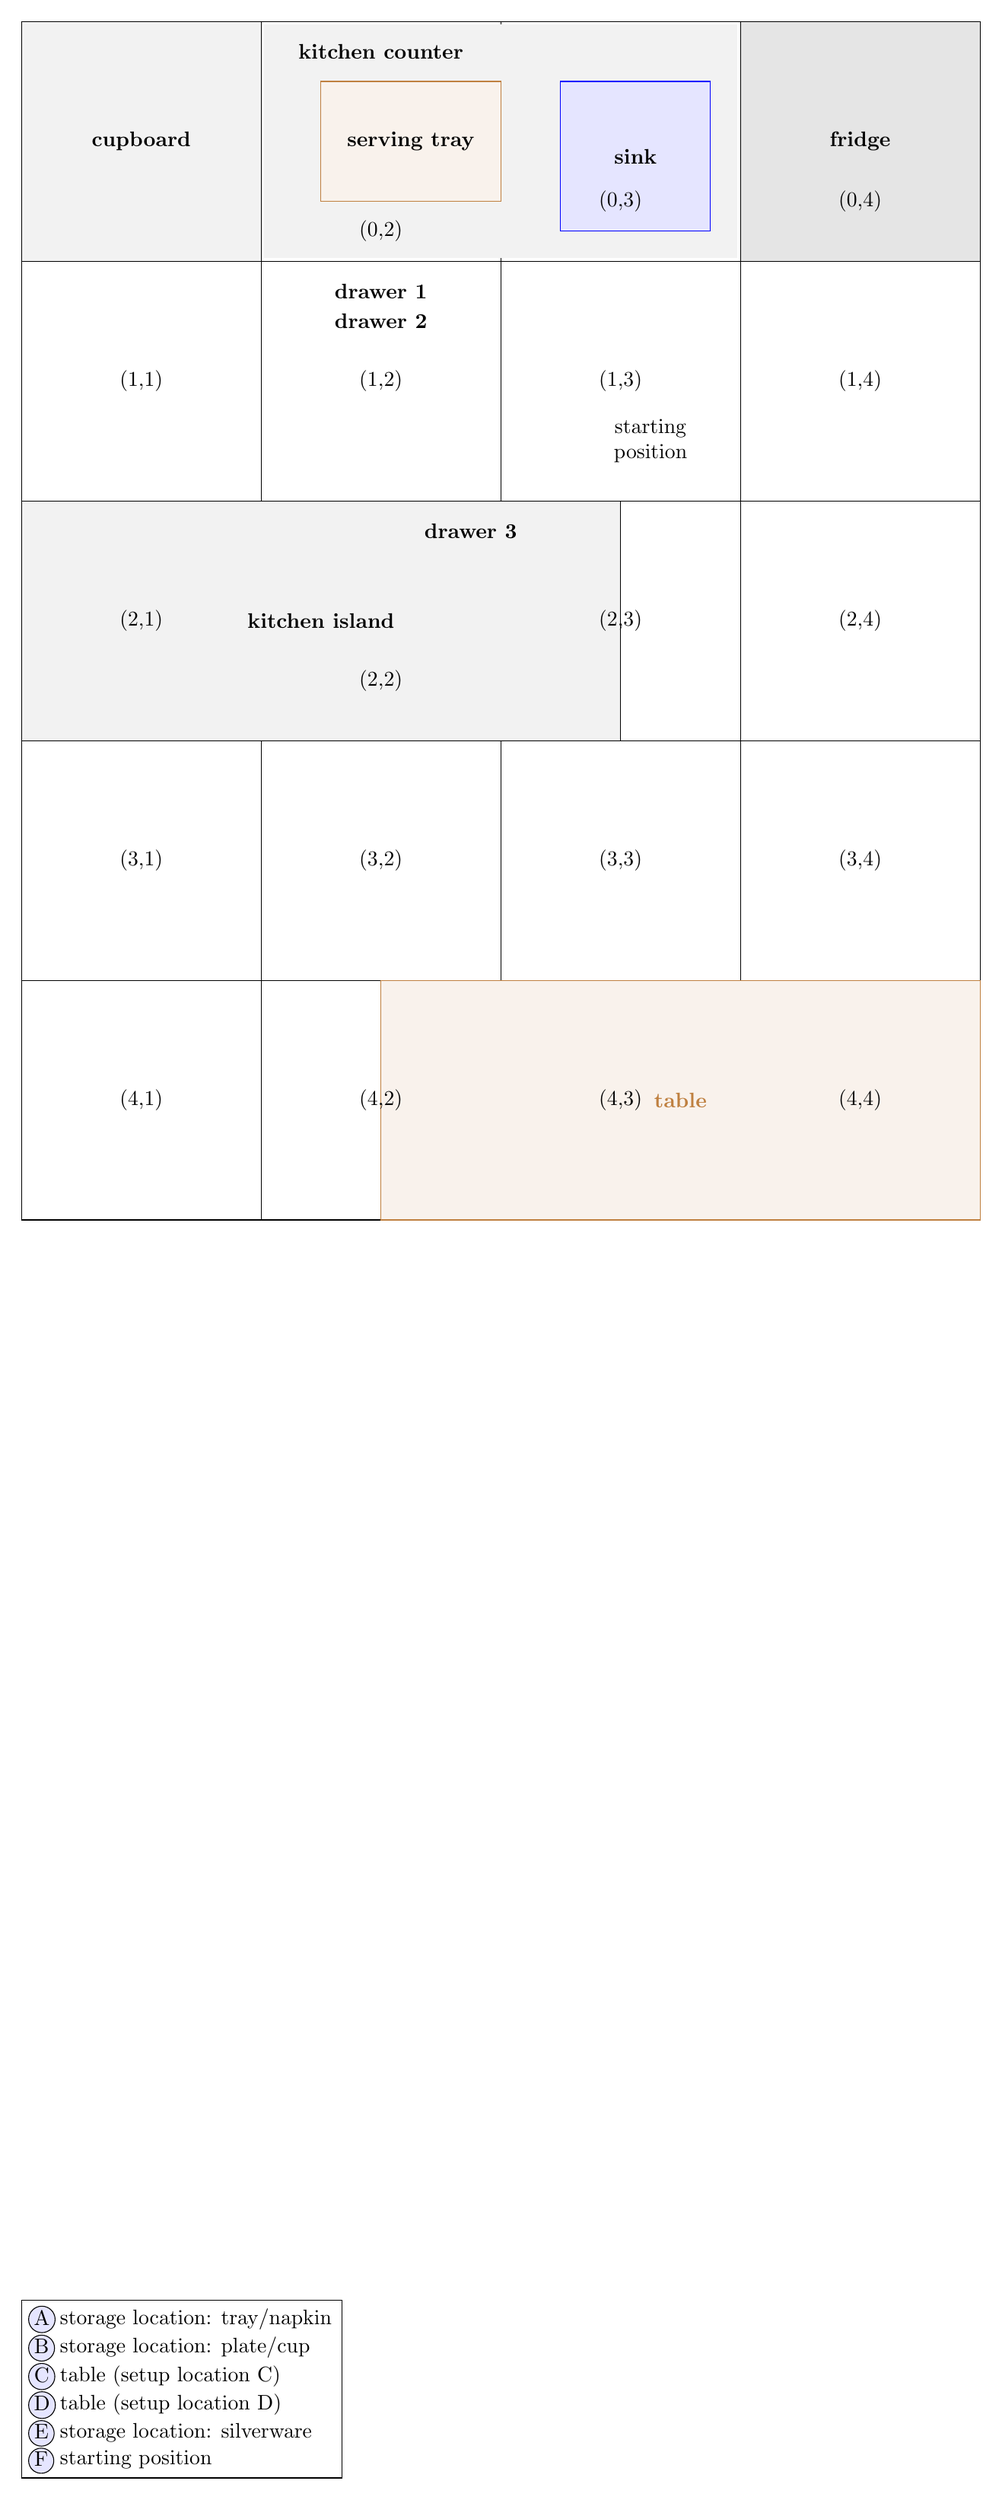
\begin{tikzpicture}
	\draw[step=4.0, black] (0,0) grid (16,20);

	\node (cupboard) [rectangle, draw=black, fill=black!5, minimum height=4cm, minimum width=4cm, align=center] (4,4) at (2,18) {\textbf{cupboard}};
	
	\draw [black] (4,0) rectangle (12,4); % node [xshift=-10ex,yshift=-8ex] {kitchen counter} (12,4);
	\node [fill=black!5!white, minimum width=7.9cm, minimum height=3.9cm] at (8,18) {};
	\node at (6,19.5) {\textbf{kitchen counter}};
	\draw [brown, fill=brown!10!white] (5,17) rectangle node [black] {\textbf{serving tray}} (8,19);
	\draw [blue, fill=blue!10!white] (9,16.5) rectangle node [black] {\textbf{sink}} (11.5,19);
	
	\node at (6,15.5) {\textbf{drawer 1}};
	\node at (6,15) {\textbf{drawer 2}};
	
	\draw [black,fill=black!10!white] (12,16) rectangle node {\textbf{fridge}} (16,20);
	
	\draw [black, fill=black!5!white] (0,8) rectangle node {\textbf{kitchen island}} (10,12);
	\node at (7.5,11.5) {\textbf{drawer 3}};
	\node[align=center] at (10.5,13) {starting\\position};
	
	%\draw [brown] (4,-12) rectangle node {table} (16,-16);
	\draw [brown,fill=brown!10!white] (6,0) rectangle node {\textbf{table}} (16,4);
	
	\node at (6,16.5) {(0,2)};
	\node at (10,17) {(0,3)};
	\node at (14,17) {(0,4)};
		
	\node at (2,14) {(1,1)};
	\node at (6,14) {(1,2)};
	\node at (10,14) {(1,3)};
	\node at (14,14) {(1,4)};
	
	\node at (2,10) {(2,1)};	
	\node at (6,9) {(2,2)};
	\node at (10,10) {(2,3)};
	\node at (14,10) {(2,4)};
	
	\node at (2,6) {(3,1)};	
	\node at (6,6) {(3,2)};
	\node at (10,6) {(3,3)};
	\node at (14,6) {(3,4)};
	
	\node at (2,2) {(4,1)};	
	\node at (6,2) {(4,2)};
	\node at (10,2) {(4,3)};
	\node at (14,2) {(4,4)};

	
	% set up legend entries
	\begin{legend}[legend cell align=left, 
	legend entries={
		storage location: tray/napkin, 
		storage location: plate/cup, 
		table (setup location C),
		table (setup location D), 
		storage location: silverware, 
		starting position}, 
	legend style={at={(0,-21)}, anchor=south west}]
	\addlegendimage{letter in legend=A, black}
	\addlegendimage{letter in legend=B, black}
	\addlegendimage{letter in legend=C, black}
	\addlegendimage{letter in legend=D, black}
	\addlegendimage{letter in legend=E, black}
	\addlegendimage{letter in legend=F, black}
	\end{legend}

\end{tikzpicture}


\end{document}